% !TeX encoding = windows-1251
\documentclass[a4paper,12pt]{article}
\usepackage{newlistok}
\usepackage{tikz}

\УвеличитьВысоту{2.5cm}
\УвеличитьШирину{1.5cm}
%\renewcommand{\spacer}{\vfil}

\Заголовок{Самостоятельная работа}
\def\словоЛисток{СР \No\/}
\НомерЛистка{1}
\ДатаЛистка{06 октября 2012г.}
\ДатаЛистка{30 января 2013г.}

\begin{document}


\ncopy{2}{
\vspace*{-12mm}
\СоздатьЗаголовок

\putthere{170mm}{-17mm}{%
    %
    %Картина для сумм треугольных чисел и т.п.
    %
      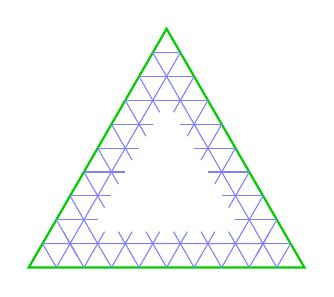
\begin{tikzpicture}
      [scale=.35
      ,fil/.style={color=green!50!white,opacity=.5}
      ,lin/.style={color=green!80!black,thick}
      ,lindot/.style={color=blue!50}
      ]
        \draw[lin] (0, 0) -- (10,0) -- ++(120:10) -- cycle;
        \foreach \i in {1,9}{
          \draw[lindot] (\i, 0) -- ++(60:10-\i);
          \draw[lindot] (\i, 0) -- ++(120:\i) -- ++(10-\i,0);
        }
        \foreach \i in {1,9}{
        }
        \foreach \i in {2,3,...,8}{
          \draw[lindot] (\i, 0) -- ++(60:1.5);
          \draw[lindot] (\i, 0) -- ++(120:1.5);
          \draw[lindot] (60:\i) -- ++(1.5,0);
          \draw[lindot] (60:\i) -- ++(-60:1.5);
          \draw[lindot] (10,0)++(120:\i) -- ++(-120:1.5);
          \draw[lindot] (10,0)++(120:\i) -- ++(-180:1.5);
        }
      \end{tikzpicture}
}{7cm}{}
\vspace{-4mm}


\УстановитьГраницы{0mm}{4truecm}
\задача
  Каждую сторону правильного треугольника разбили на $n$ частей и через точки деления провели прямые, параллельные сторонам треугольника. На сколько частей оказался разбит треугольник?
\кзадача


\задача
  На контрольной работе по математическому анализу было четыре задачи. За каждую задачу можно получить либо \лк $+$\пк, либо \лк $-$\пк. Правда ли, что результаты каких-нибудь двух школьников обязательно совпадут, если в классе 19 человек?
\кзадача
\ВосстановитьГраницы

\задача
  Сколькими способами можно выбрать четырёх дежурных в гардероб из 19 школьников, если староста Вася обязательно должен дежурить?
\кзадача


\задача
  В геометрической прогрессии 57 членов, причём первый и последний равны $1$.
  Чему может быть равна сумма всех 57 её членов?
\кзадача

\vspace*{-4mm}
\допраздел{* * *}
\vspace*{-2mm}

\сзадача
  В цветочном магазине продаются цветы 10 сортов. Сколько разных букетов из трёх (не обязательно различных) цветков можно составить?
\кзадача
\hrl
\note{Для получения оценки $n$ необходимо правильно решить $n-1$ задачу. Решившие все 5 задач получают две пятёрки.\\
Пользоваться листками, своими записями и т.д. нельзя. Задачи необходимо \выд качественно записать. }
}


%\ЛичныйКондуит{0mm}{6mm}
%\СделатьКондуит{6mm}{6mm}

\end{document}
